\documentclass{article}
\usepackage[utf8]{inputenc}
\usepackage[margin=1in]{geometry}
\usepackage{fancyhdr}
\usepackage{graphicx}
\usepackage{listings}
\usepackage{parskip}
\usepackage{amsmath}

\makeatletter
  \def\@seccntformat#1{\@ifundefined{#1@cntformat}
    {\csname the#1\endcsname\space}
    {\csname #1@cntformat\endcsname}}
  \newcommand\section@cntformat{\thesection.\space}       
  \newcommand\subsection@cntformat{\thesubsection.\space}
\makeatother

\newcommand{\code}[1]{\texttt{#1}}

\renewcommand\thesubsection{\alph{subsection}}

\title{EECS 219C: Formal Methods — Assignment 3}
\author{Parker Ziegler}
\pagestyle{fancy}
\lhead{EECS 219C: Formal Methods — Assignment 3}
\rhead{Parker Ziegler}

\begin{document}

\maketitle

\section{Interrupt-Driven Program}

\subsection{Describing properties of the \code{Sys} module}

We can describe the properties of the \code{Sys} module as follows:

\begin{enumerate}
  \item \textbf{\code{invariant main\_ISR\_mutex}} — this property requires that execution of \code{main} and \code{ISR} is mutually exclusive. That is, if \code{main} is executing, \code{ISR} cannot be executing at the same time (or vice versa).
  \item \textbf{\code{property[LTL] one\_step\_ISR\_return}} — this property requires that, globally, if \code{ISR} has just returned then, in the next state, \code{ISR} will not return.
  \item \textbf{\code{property[LTL] main\_after\_ISR}} — this property requires that, globally, if \code{ISR} is currently enabled to run and, in the next state, \code{main} is enabled to run, this implies that \code{ISR} has just returned.
  \item \textbf{\code{property[LTL] ISR\_after\_main}} — this property requires that, globally, if \code{main} is enabled and, in the next state, \code{ISR} is enabled, this implies that an interrupt has occurred.
\end{enumerate}

\subsection{Interpreting counterexamples from the verifier}

Running \code{uclid} with all properties commented out \emph{except} for \code{main\_after\_ISR} results in the following counterexample:

\begin{lstlisting}
CEX for vobj [Step #3] property main_after_ISR:safety @ IntSW.ucl, line 105
=================================
Step #0
  mode : main_t
  M_enable : true
  I_enable : false
  return_ISR : false
  assert_intr : initial_1570_assert_intr
=================================
=================================
Step #1
  mode : ISR_t
  M_enable : true
  I_enable : false
  return_ISR : false
  assert_intr : false
=================================
=================================
Step #2
  mode : main_t
  M_enable : false
  I_enable : true
  return_ISR : false
  assert_intr : false
=================================
=================================
Step #3
  mode : main_t
  M_enable : true
  I_enable : false
  return_ISR : false
  assert_intr : false
=================================

// Steps 4 and step 5 elided.

Finished execution for module: Sys.
\end{lstlisting}

In this counterexample, the violation of \code{main\_after\_ISR} occurs between step 2 and step 3 of the transition system. At step 2, we see that \code{I\_enable} is set to $true$ and \code{M\_enable} is set to $false$, indicating that \code{ISR} is enabled to run. Additionally, the value of \code{return\_ISR} is $false$, indicating that \code{ISR} has not yet returned. In the next step, \code{I\_enable} is $false$ and \code{M\_enable} is $true$; this indicates that \code{ISR} should have completed running and \code{main} can safely be enabled. However, \code{return\_ISR} is still $false$. In this instance, we have a case where \code{ISR} \emph{was enabled}, but we have no indication that it ever returned before \code{main} was enabled. This violates the property that if \code{ISR} was enabled and, in the next state, \code{main} is enabled, then \code{return\_ISR} \emph{must} be $true$.

Running \code{uclid} with all properties commented out \emph{except} for \code{ISR\_after\_main} results in the following counterexample:

\begin{lstlisting}
CEX for vobj [Step #2] property ISR_after_main:safety @ IntSW.ucl, line 106
=================================
Step #0
  mode : main_t
  M_enable : true
  I_enable : false
  return_ISR : false
  assert_intr : false
=================================
=================================
Step #1
  mode : ISR_t
  M_enable : true
  I_enable : false
  return_ISR : false
  assert_intr : false
=================================
=================================
Step #2
  mode : main_t
  M_enable : false
  I_enable : true
  return_ISR : false
  assert_intr : false

// Steps 3, 4, and 5 elided.

Finished execution for module: Sys.
\end{lstlisting}

In this counterexample, the violation of \code{ISR\_after\_main} occurs between step 1 and step 2 of the transition system. At step 1, we see that \code{M\_enable} is set to $true$ while \code{I\_enable} is set to $false$, indicating we are in the \code{ISR} function. In step 2, \code{I\_enable} is $true$, \code{M\_enable} is $false$, indicating we moved execution to the \code{main} function. This second state would imply that an interrupt has been issued; however, \code{assert\_intr} is $false$. This indicates that we transitioned into enabling \code{ISR} without an interrupt ever occurring. This violates the property that, if \code{main} is enabled in the current state and, in the next state, \code{ISR} is enabled, then \code{assert\_intr} \emph{must} be $true$.

\subsection{Correctly composing \code{main} and \code{ISR}}

See my updated definition of the \code{update\_mode} procedure in \code{Int\_SW.ucl}.

\subsection{Composing \code{Sys} and \code{Env} using asynchronous composition with interleaving semantics}

See my updates to the \code{init} and \code{next} blocks of the \code{main} module in \code{Int\_SW.ucl}.

The key change introduced in my updates is ensuring that \code{turn} is non-deterministically updated in the \code{init} and \code{next} blocks of the \code{main} module using \code{havoc}. In an asynchronous composition of \code{Sys} and \code{Env} with interleaving semantics, either \code{Sys} can transition and \code{Env} stutters, or \code{Env} can transition and \code{Sys} stutters:

\begin{align*}
(\delta((Sys, Env), (Sys', Env')) &= \delta(Sys, Sys') \land Env = Env) \lor \\
(\delta((Sys, Env), (Sys', Env')) &= Sys = Sys \land \delta(Env, Env'))
\end{align*}

Importantly, \emph{which} of these entities transitions in a given step is non-deterministic. For example, we could have a model where only \code{Sys} ever transitions or only \code{Env} ever transitions.

This composition does lead to a violation of the \code{consec\_main\_pc\_values} LTL property. \code{uclid} provides a counterexample in which only \code{Env} ever transitions. In this case, the \code{main} function is always at its initial program counter $A$ but, because \code{Sys} never runs, it never transitions to program counter $B$. This violates the property that, at some point in the future, \code{main} will transition from program counter $A$ to program counter $B$.

\section{Smart Intersection}

\subsection{Encoding the \code{no\_collision} invariant}

In our modeled intersection, we encode collisions as situations in which two of our autonomous vehicles are in the same location in the intersection. To do this, we use pairwise location comparisons between all vehicles. These can be enumerated as follows:

\begin{enumerate}
  \item If \code{car1\_pos} and \code{car2\_pos} are in the intersection, this implies that \code{car1\_pos} is not equal to \code{car2\_pos}.
  \item If \code{car2\_pos} and \code{car3\_pos} are in the intersection, this implies that \code{car2\_pos} is not equal to \code{car3\_pos}.
  \item If \code{car1\_pos} and \code{car3\_pos} are in the intersection, this implies that \code{car1\_pos} is not equal to \code{car3\_pos}.
\end{enumerate}

The formal encoding of our \code{no\_collision} invariant is:

\begin{lstlisting}
invariant no_collision: (
  (in_intersection(car1_pos) && in_intersection(car2_pos) ==> car1_pos != car2_pos) &&
  (in_intersection(car2_pos) && in_intersection(car3_pos) ==> car2_pos != car3_pos) &&
  (in_intersection(car1_pos) && in_intersection(car3_pos) ==> car1_pos != car3_pos)
);
\end{lstlisting}

This invariant is stronger than just doing pairwise comparisons of car locations. A "collision" should be restricted to only occurring within an intersection. Since cars are respawned at source locations non-deterministically, we don't consider two cars at the same source as a "collision".

\subsection{Defining the \code{can\_move} procedure}

To determine whether or not a car can move, we use an algorithm that gives priority to cars that are currently in the intersection over cars that are at a source location. The algorithm begins by first checking if a car is at a sink location or if it's currently in the intersection. If the car is at a sink location, we immediately set its \code{move} flag to $true$, because it must move to (respawn at) a source location in the next step. If the car is in the intersection, we also set its \code{move} flag to $true$, giving it "priority" over cars still at source locations.

We then handle cars at source locations. We only allow a car at a source location to move if its next location (computed by calling the \code{next\_location} procedure with a $steps$ argument of 1) is not equal to the next locations of the other two cars. In other words, we only allow a car at source locations to move if cars currently in the intersection will not occupy the same location in the next step.

\subsection{Encoding the \code{bounded\_exit} invariant}

In order to ensure that each car exits the intersection in a bounded number of steps, we simply check that its \code{wait\_count} does not exceed the total number of steps taken in the bounded model checking process.

\begin{lstlisting}
  invariant bounded_exit: wait_cnt1 < 16 && wait_cnt2 < 16 && wait_cnt3 < 16;
\end{lstlisting}

A car's wait count is incremented on every transition of the system as long as it hasn't reached a sink location. Therefore, if a car's wait count reached the number of steps of the bounded model checking process, this would imply that the car was either stuck at a source location or in the intersection.

\subsection{Induction proof}

\code{uclid} was able to construct an inductive proof using our definition of the \code{no\_collision} invariant and implementation of the \code{can\_move} procedure without any additional strengthening invariants.

\section{Linear Temporal Logic (LTL)}

\subsection{A labeled transition system for Sisyphus' task}

To define a labeled transition system for Sisyphus' task, we must define the constituent parts of our transition system. Recall that a labeled transition system, or Kripke structure, takes the form:

$$
(S, S_0, \delta, L)
$$

In order to define our set of states $S$ and initial state $S_0$, we need to define the variables that make up our state. We'll use four Boolean valued variables to represent our four entities, each with a value of 0 or 1 indicating whether they are on the western bank of the river (start) or the eastern bank of the river (end):

\begin{enumerate}
  \item \code{s} — Sisyphus' location 
  \item \code{g} — the goat's location
  \item \code{w} — the wolf's location
  \item \code{c} — the cabbage's location
\end{enumerate}

Our initial state $S_0$ can then be described by the set $\{s = 0, g = 0, w = 0, c = 0\}$. Our set of states $S$ is the set of all Boolean combinations of these states, such that two invariants hold: 

\begin{enumerate}
  \item $w = g \Longrightarrow w = g = s$ — if the wolf and goat are on the same side, then Sisyphus must also be on that side.
  \item $c = g \Longrightarrow c = g = s$ — if the cabbage and goat are on the same side, then Sisyphus is not on that side.
\end{enumerate}

In this system, a transition $\delta$ involves flipping the values of at most two entities, one of which must be $s$. This reflects the constraint that the boat only has room for at most two entities, one of which must be Sisyphus himself.

Finally, our labeling function defines all possible transitions of this system. We represent this using a labeled finite state automata in Figure \ref{fig:ltl-automata} In this automata, we use the notation $W:<s | g | w | c>$ and $E:<s | g | w | c>$ to label the state at each node. For example, the state in which the wolf $w$ is on the western bank and Sisyphus, the goat, and the cabbage are on the eastern bank is notated as $W: w, E: sgc$. We also label the transition relation $\delta$ as a set of updates that take place at an edge between two states.

\begin{figure}
  \centering
  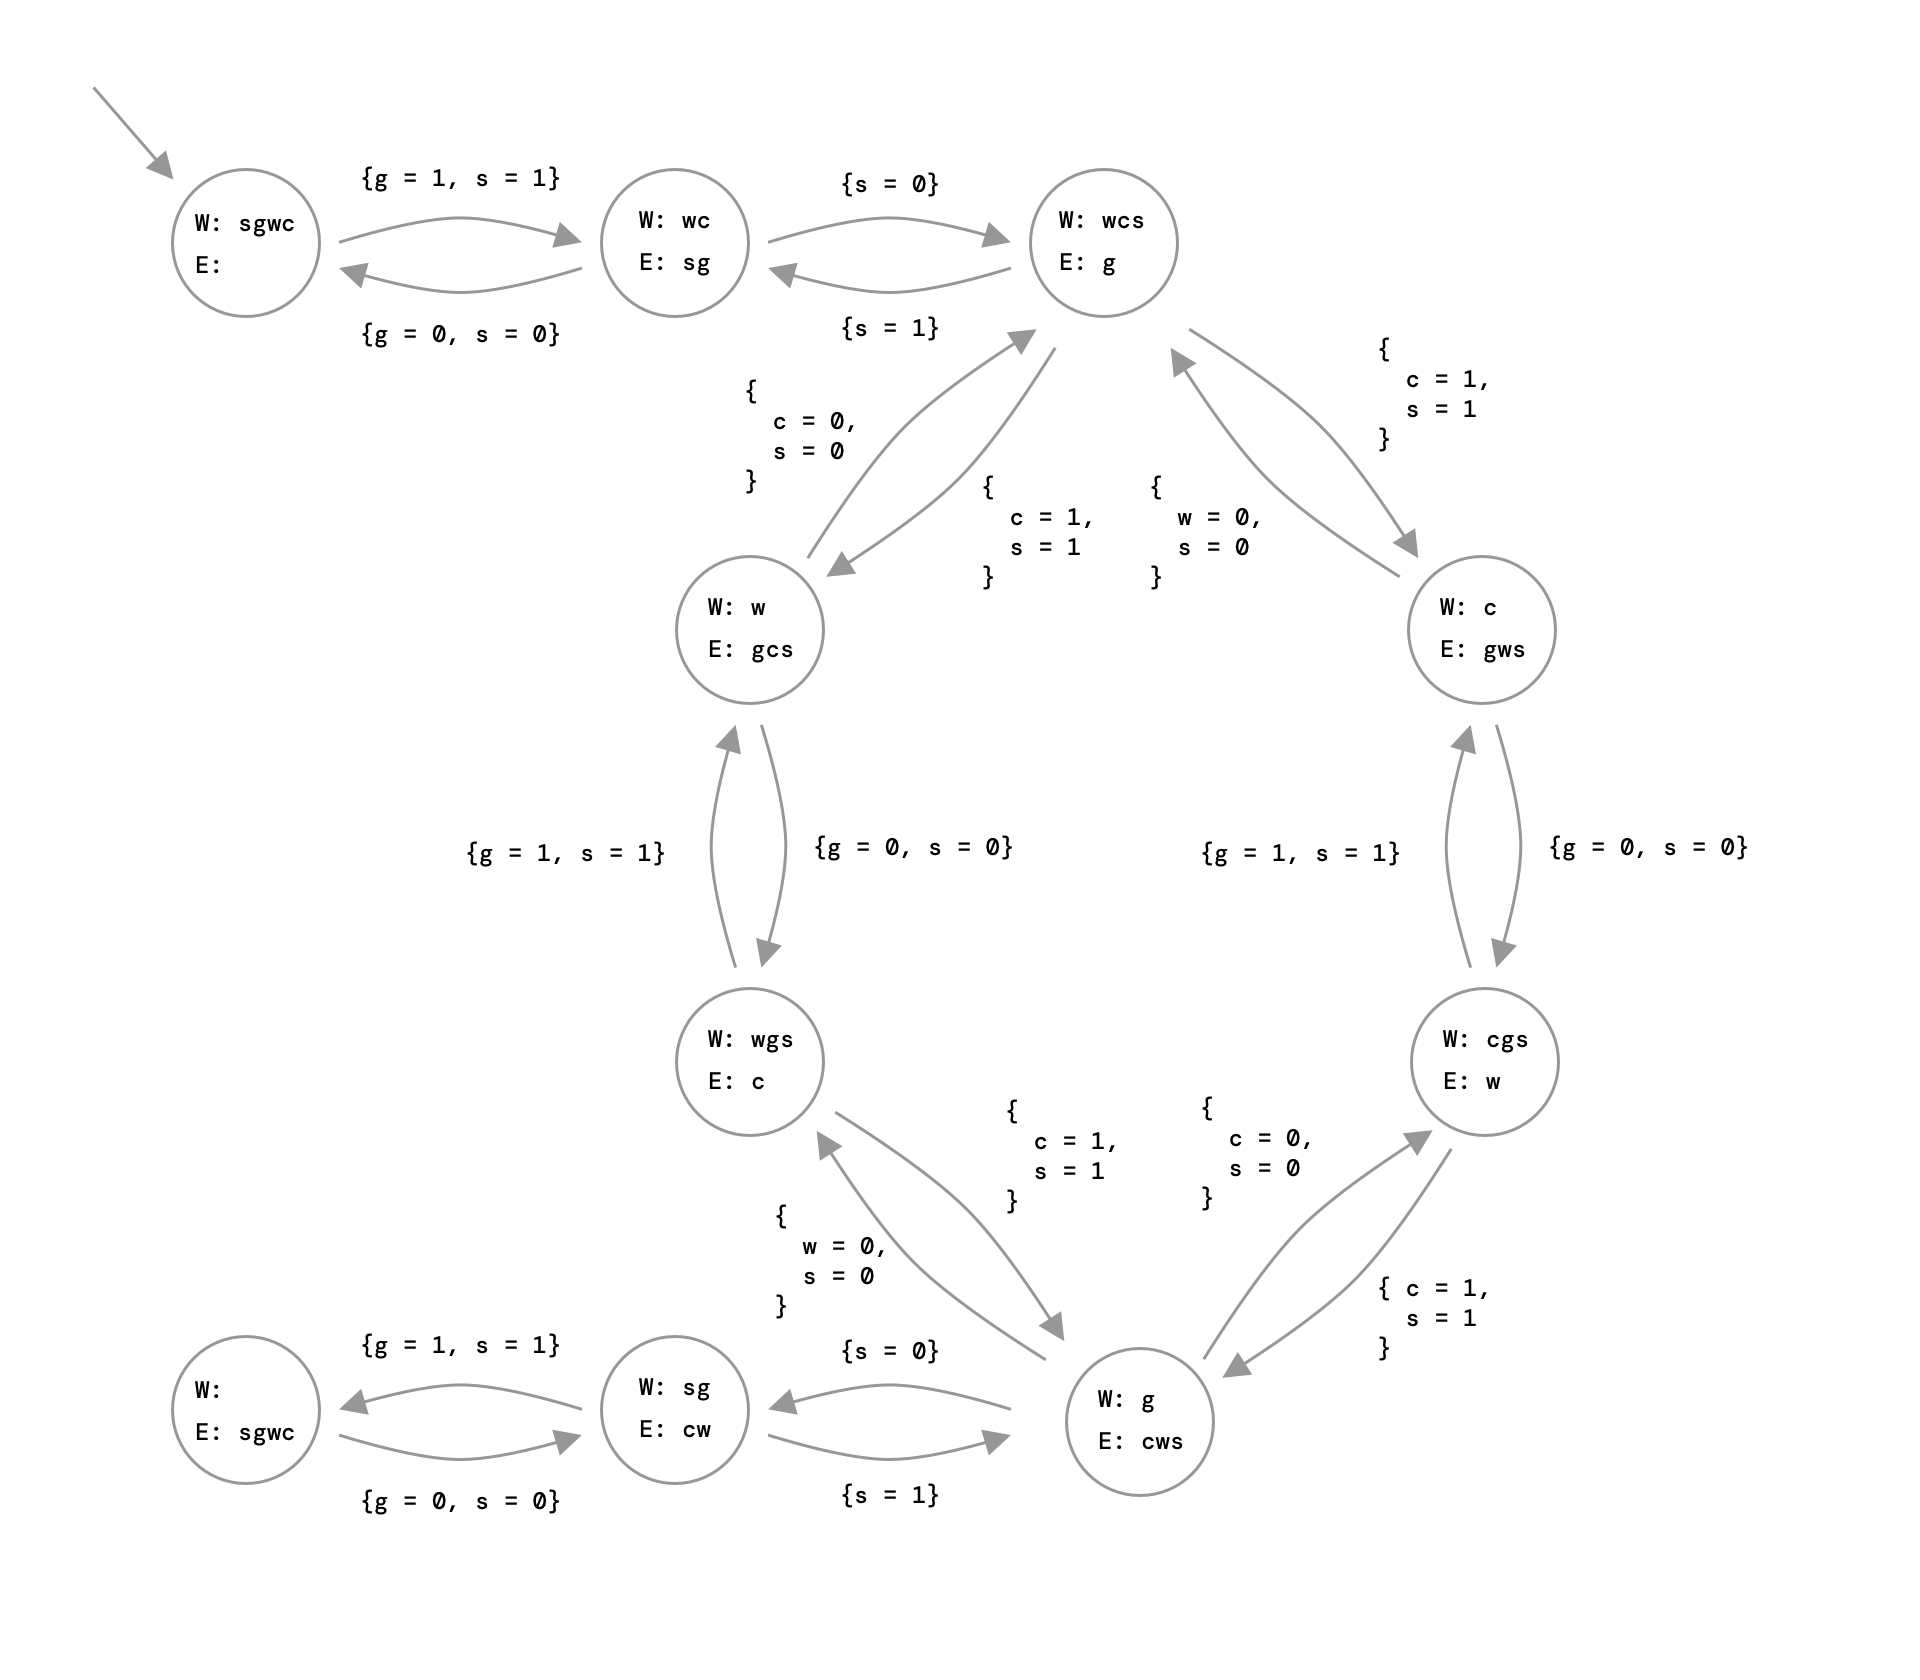
\includegraphics[width=0.9\textwidth]{ltl-automata}
  \caption{The labeled transition system encoding the river crossing problem.}
  \label{fig:ltl-automata}
\end{figure}

\subsection{LTL formula for Sisyphus' task}

To define LTL formula for Sisyphus' task and the constraints that the goat / wolf and goat / cabbage not be left alone on the same bank, we use the same variables defined above.

Let us now describe the reasoning for our LTL formula. First, we know that if the cabbage and the goat are on the same side ($c = g$), then Sisyphus must be on that side as well ($c = g \Longrightarrow c = g = s$). Likewise, if the goat and the wolf are on the same side ($g = w$), then Sisyphus must be on that side as well ($g = w \Longrightarrow g = w = s$). Notice that the goat, $g$, appears twice in these constraints. Combining these together, we can arrive at the following LTL formula:

$$
G(c = g \lor w = g \Longrightarrow g = s)
$$

Concretely, this formula states that, globally, if the cabbage and the goat are on the same bank or if the goat and the wolf are on the same bank, then Sisyphus \emph{must} be on the same bank as the goat.

We could additionally add the formula specifying that, eventually, all entities will be on the opposite side of the river. Since we start with all entities on the western bank ($s = g = w = c = 0$), we want to verify that all entities eventually reach the eastern bank. We can encode this using the future operator $F$ as follows:

$$
F(s = g = w = c = 1)
$$

Conjuncting all of these together, we arrive at:

$$
G(c = g \lor w = g \Longrightarrow g = s) \land F(s = g = w = c = 1)
$$

\subsection{A solution to Sisyphus' task}

Uncovering a solution to Sisyphus' task relies on making one key observation: there is no restriction stating that Sisyphus cannot \emph{return} items to the opposing bank during the transport of all three items from one bank to the other. With this observation, the following procedure solves Sisyphus' task:

\begin{enumerate}
  \item Assume all items are on the western bank to start — $s = 0, g = 0, w = 0, c = 0$.
  \item Bring the goat to the eastern bank — $s = 1, g = 1, w = 0, c = 0$.
  \item Return to the western bank — $s = 0, g = 1, w = 0, c = 0$.
  \item Bring the wolf to the eastern bank — $s = 1, g = 1, w = 1, c = 0$.
  \item Return to the western bank \emph{with the goat} — $s = 0, g = 0, w = 1, c = 0$.
  \item Bring the cabbage to the eastern bank — $s = 1, g = 0, w = 1, c = 1$.
  \item Return to the western bank — $s = 0, g = 0, w = 1, c = 1$.
  \item Bring the goat to the eastern bank — $s = 1, g = 1, w = 1, c = 1$.
\end{enumerate}

\subsection{Creating a Spin model for the river crossing problem}

My encoding of a Spin model for the river crossing problem can be found in \code{river\_crossing.pml}.

\subsection{Showing model satisfaction of LTL formula for the river crossing problem}

My encoding of LTL formula for the river crossing problem can be found in \code{river\_crossing.pml}.

\end{document}